% -*- coding: utf-8 -*-
\documentclass[UTF8,a4paper,10pt]{ctexart}
\usepackage[left=3.17cm, right=3.17cm, top=2.74cm, bottom=2.74cm]{geometry}
\usepackage{amsmath}
\usepackage{graphicx,subfig}
\usepackage{float}
\usepackage{cite}
\usepackage{caption}
\usepackage{enumerate}
\usepackage{booktabs} %表格
\usepackage{multirow}
\newcommand{\tabincell}[2]{\begin{tabular}{@{}#1@{}}#2\end{tabular}}  %表格强制换行
%-------------------------字体设置--------------
% \usepackage{times} 
\usepackage{ctex}
\setCJKmainfont[ItalicFont=Noto Sans CJK SC Bold, BoldFont=Noto Serif CJK SC Black]{Noto Serif CJK SC}


\newcommand{\yihao}{\fontsize{26pt}{36pt}\selectfont}           % 一号, 1.4 倍行距
\newcommand{\erhao}{\fontsize{22pt}{28pt}\selectfont}          % 二号, 1.25倍行距
\newcommand{\xiaoer}{\fontsize{18pt}{18pt}\selectfont}          % 小二, 单倍行距
\newcommand{\sanhao}{\fontsize{16pt}{24pt}\selectfont}  %三号字
\newcommand{\xiaosan}{\fontsize{15pt}{22pt}\selectfont}        % 小三, 1.5倍行距
\newcommand{\sihao}{\fontsize{14pt}{21pt}\selectfont}            % 四号, 1.5 倍行距
\newcommand{\banxiaosi}{\fontsize{13pt}{19.5pt}\selectfont}    % 半小四, 1.5倍行距
\newcommand{\xiaosi}{\fontsize{12pt}{18pt}\selectfont}            % 小四, 1.5倍行距
\newcommand{\dawuhao}{\fontsize{11pt}{11pt}\selectfont}       % 大五号, 单倍行距
\newcommand{\wuhao}{\fontsize{10.5pt}{15.75pt}\selectfont}    % 五号, 单倍行距
%-------------------------章节名----------------
\usepackage{ctexcap} 
\CTEXsetup[name={,、},number={ \chinese{section}}]{section}
\CTEXsetup[name={(,)},number={\chinese{subsection}}]{subsection}
\CTEXsetup[name={,.},number={\arabic{subsubsection}}]{subsubsection}
%-------------------------页眉页脚--------------
\usepackage{fancyhdr}
\pagestyle{fancy}
\lhead{\kaishu \leftmark}
% \chead{}
\rhead{\kaishu 计算机网络实验报告}
\lfoot{}
\cfoot{\thepage}
\rfoot{}
\renewcommand{\headrulewidth}{0.1pt}  
\renewcommand{\footrulewidth}{0pt}%去掉横线
\newcommand{\HRule}{\rule{\linewidth}{0.5mm}}%标题横线
\newcommand{\HRulegrossa}{\rule{\linewidth}{1.2mm}}
%-----------------------伪代码------------------
\usepackage{algorithm}  
\usepackage{algorithmicx}  
\usepackage{algpseudocode}  
\floatname{algorithm}{Algorithm}  
\renewcommand{\algorithmicrequire}{\textbf{Input:}}  
\renewcommand{\algorithmicensure}{\textbf{Output:}} 
\usepackage{lipsum}  
\makeatletter
\newenvironment{breakablealgorithm}
  {% \begin{breakablealgorithm}
  \begin{center}
     \refstepcounter{algorithm}% New algorithm
     \hrule height.8pt depth0pt \kern2pt% \@fs@pre for \@fs@ruled
     \renewcommand{\caption}[2][\relax]{% Make a new \caption
      {\raggedright\textbf{\ALG@name~\thealgorithm} ##2\par}%
      \ifx\relax##1\relax % #1 is \relax
         \addcontentsline{loa}{algorithm}{\protect\numberline{\thealgorithm}##2}%
      \else % #1 is not \relax
         \addcontentsline{loa}{algorithm}{\protect\numberline{\thealgorithm}##1}%
      \fi
      \kern2pt\hrule\kern2pt
     }
  }{% \end{breakablealgorithm}
     \kern2pt\hrule\relax% \@fs@post for \@fs@ruled
  \end{center}
  }
\makeatother
%------------------------代码-------------------
\usepackage{xcolor} 
\usepackage{listings} 
\usepackage{graphicx}
\lstset{ 
breaklines,%自动换行
basicstyle=\small,
escapeinside=``,
keywordstyle=\color{ blue!70} \bfseries,
commentstyle=\color{red!50!green!50!blue!50},% 
stringstyle=\ttfamily,% 
extendedchars=false,% 
linewidth=\textwidth,% 
numbers=left,% 
numberstyle=\tiny \color{blue!50},% 
frame=trbl% 
rulesepcolor= \color{ red!20!green!20!blue!20} 
}
%------------超链接----------
\usepackage[colorlinks,linkcolor=black,anchorcolor=blue]{hyperref}
%------------------------TODO-------------------
\usepackage{enumitem,amssymb}
\newlist{todolist}{itemize}{2}
\setlist[todolist]{label=$\square$}
% for check symbol 
\usepackage{pifont}
\newcommand{\cmark}{\ding{51}}%
\newcommand{\xmark}{\ding{55}}%
\newcommand{\done}{\rlap{$\square$}{\raisebox{2pt}{\large\hspace{1pt}\cmark}}\hspace{-2.5pt}}
\newcommand{\wontfix}{\rlap{$\square$}{\large\hspace{1pt}\xmark}}
%------------------------水印-------------------
\usepackage{tikz}
\usepackage{xcolor}
\usepackage{eso-pic}
\usepackage{verbatim}

\newcommand{\watermark}[3]{\AddToShipoutPictureBG{
\parbox[b][\paperheight]{\paperwidth}{
\vfill%
\centering%
\tikz[remember picture, overlay]%
  \node [rotate = #1, scale = #2] at (current page.center)%
    {\textcolor{gray!80!cyan!30!magenta!30}{#3}};
\vfill}}}
\lstset{
  basicstyle=\ttfamily\small, % 使用打字机字体并设置为小号
  numbers=left,
}
%———————————————————————————————————————————正文
%----------------------------------------------
\begin{document}
\begin{titlepage}
    \begin{center}
    
\includegraphics[width=0.8\textwidth]{NKU.png}\\[1cm]    
    \textsc{\Huge \kaishu{\textbf{南\ \ \ \ \ \ 开\ \ \ \ \ \ 大\ \ \ \ \ \ 学}} }\\[0.9cm]
    \textsc{\huge \kaishu{\textbf{网\ \ 络\ \ 空\ \ 间\ \ 安\ \ 全\ \ 学\ \ 院}}}\\[0.9cm]
    \textsc{\huge \kaishu{\textbf{计算机网络实验报告}}}\\[0.8cm]
    \HRule \\[0.9cm]
    { \LARGE \bfseries Lab3-4 性能对比}\\[0.4cm]
    \HRule \\[2.0cm]
    \centering
    \textsc{\LARGE \kaishu{2113946\ \ \ 刘国民 }}\\[0.5cm]
    \textsc{\LARGE \kaishu{年级\ :\ 2021级}}\\[0.5cm]
    \textsc{\LARGE \kaishu{专业\ :\ 信息安全}}\\[0.5cm]
    \vfill
    {\Large \today}
    \end{center}
\end{titlepage}



\newpage
\tableofcontents
\setcounter{page}{1}

\vspace{1cm}

\section{实验内容}
本次实验在已实现的3次基于UDP的可靠传输实验基础上,通过调节丢包率和延时等参数获得不同的性能,并对实验结果进行分析和解释。在实验3-3(选择确认)中,我删除了接收方回复ACK包的数据缓冲区以减少实际的数据传输大小,在本次实验中为保证公平性,均采用一致的报文格式,传输文件以1.jpg为例,由于文件大小固定,这里我们只比较吞吐率即可。
\vspace{1cm}

\section{停等机制与滑动窗口机制性能对比}
这里将实验3-2(滑动窗口)和实验3-1(停等机制)进行比较。固定滑动窗口大小为4。我们首先固定延时为0ms,改变丢包率。具体测试数据如下:
\begin{table}[h!]
  \centering
  \begin{tabular}{|l|c|r|} % l=left, c=center, r=right
    \hline
     丢包率   & 停等机制    & 滑动窗口 \\ \hline
    0\% & 11.008Mbps & 1.418Mbps \\ \hline
    2\% & 0.415Mbps & 0.239Mbps \\ \hline
    4\% & 0.265Mbps & 0.161Mbps \\ \hline
    6\% & 0.214Mbps & 0.106Mbps \\ \hline
    8\% & 0.168Mbps & 0.083Mbps \\ \hline
    10\% & 0.136Mbps & 0.061Mbps \\ \hline
  \end{tabular}
  \caption{停等机制与滑动窗口的吞吐率对比}
  \label{tab:my_label}
\end{table}\par
将数据绘制成统计图:
\begin{figure}[H]
    \centering
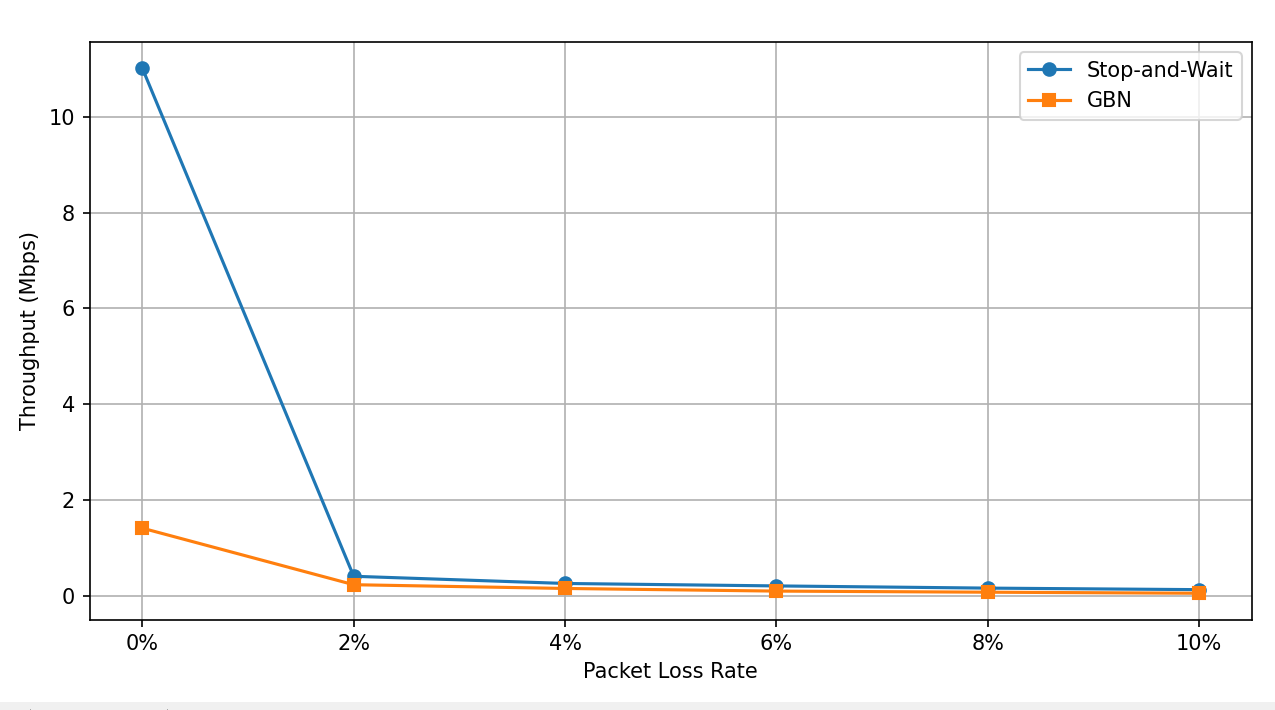
\includegraphics[width=0.8\textwidth]{img/p1-1.png}
    \caption{停等协议 vs 滑动窗口}
\end{figure}
固定丢包率为0,之后改变延时。
\begin{table}[h!]
  \centering
  \begin{tabular}{|l|c|r|} % l=left, c=center, r=right
    \hline
  延时    & 停等机制    & 滑动窗口      \\ \hline
  0ms	   & 11.008Mbps & 1.418Mbps    \\ \hline
  5ms	   & 0.505Mbps	& 0.451Mbps    \\ \hline
 10ms	& 0.437Mbps  & 0.405Mbps    \\ \hline
 20ms	& 0.399Mbps  & 0.327Mbps    \\ \hline  
 40ms	& 0.321Mbps	 & 0.287Mbps    \\ \hline
 60ms	& 0.268Mbps	 & 0.256Mbps    \\ \hline
 80ms	& 0.246Mbps  & 0.220Mbps    \\ \hline
100ms	 & 0.214Mbps  & 0.178Mbps    \\ \hline
  \end{tabular}
  \caption{停等机制与滑动窗口的吞吐率对比}
  \label{tab:my_label}
\end{table}\par
延时的统计图,这里省略了 0ms 的数据。
\begin{figure}[H]
    \centering
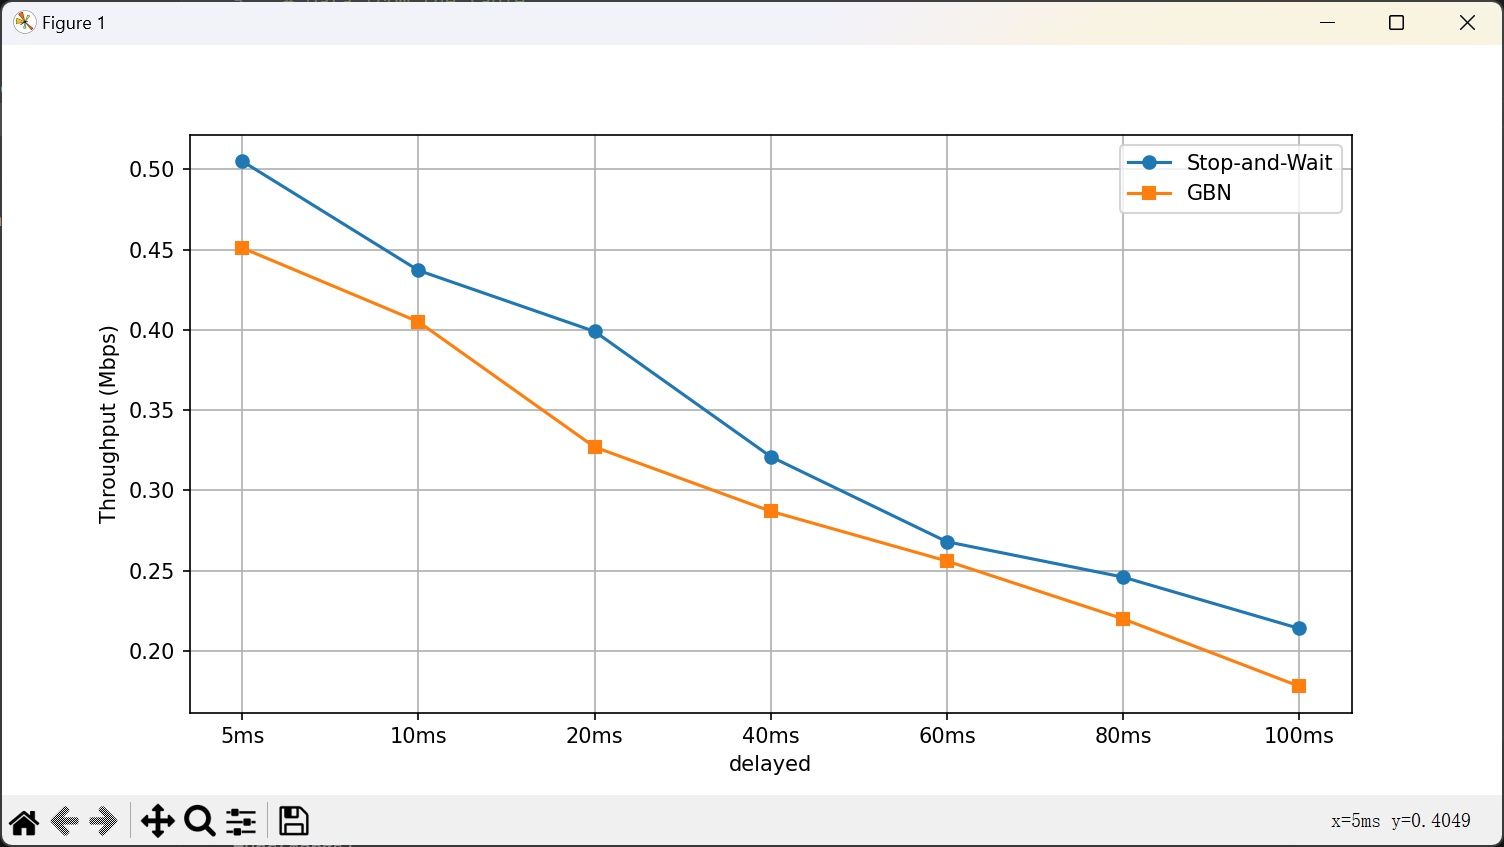
\includegraphics[width=0.8\textwidth]{img/p1-2.png}
    \caption{停等协议 vs 滑动窗口}
\end{figure}
这里出现了与理论课内容相违背的结果。即在同一丢包率和延时下,停等协议传输吞吐率均优于滑动窗口机制。本着实事求是的态度,我们还是如实使用原始数据。但这与理论课讲授的结论是相反的。按照徐老师讲述的内容,停等机制中发送端在正确收到 ACK 回复后才会发出下一个数据包。链路利用率较低,因此引入流水线和滑动窗口机制来发送多个包,即在确认未返回之前允许发送多个分组。实验中尽管我已经删除了 cout 等I/O调度比较耗时的日志输出信息,但测试下来滑动窗口仍然比停等协议慢很多。理论上来说,发送端依据状态机模型,针对不同时间完成不同的响应即可。但在实际代码编写中,我发现在主线程 main 之外,还需要一个线程来负责接收 ACK,同时超时之后还需要重传数据。使用单线程面向过程的编程思路难以实现。因此在这个地方我单独又开了两个线程来持续 Recv 和 Resend,并通过标志位的改变来持续检测。这也意味着,需要使用全局变量来共享线程之间的标志位,意味着需要用互斥锁来保证每次读写的原子性。所以,滑动窗口机制理论上会优于停等协议,但在实际编程中(个人编程技巧太菜导致)最终吞吐率劣于停等协议。\par
同时我们可以从图表中看到,随着丢包率的升高,滑动窗口的吞吐率下降速度会快于停等协议。这是因为 3-2 使用累积确认,一旦 Base 包丢失,那么则需要重传整个窗口。随着丢包率的增加,这会造成带宽的严重浪费。(即链路上全是本来没有必要的重传数据包)所以滑动窗口吞吐率下降更快。延时增加,则两种机制吞吐率也会相应降低,这是因为延时增加后发送端传给路由器后会做相应的延时处理,从而增加每一个数据包的 RTT。停等协议或者滑动窗口收到 ACK 包的时间也会比原来相应往后延迟。此时发现两者下降趋势基本呈一条直线,且斜率基本相同。这是因为增加延时,RTT 只要没有到达设置的超时时间,每个 RTT 都线性增加。总的传输时间的增加也应线性变化。所以两者下降速率差异不大。


\section{滑动窗口机制中不同窗口大小对性能的影响}
我们分别进行测试累计确认和选择确认中不同窗口大小的影响。这里我们固定丢包率为2\%,延时为5ms,分别测试不同窗口大小下的吞吐率。图表如下:
\begin{table}[h!]
  \centering
  \begin{tabular}{|l|c|r|} % l=left, c=center, r=right
    \hline
     窗口大小   & 累计确认    & 选择确认 \\ \hline
    4  & 0.189Mbps&  0.203Mbps \\ \hline
    12 & 0.154Mbps & 0.184Mbps \\ \hline
    20 & 0.115Mbps & 0.167Mbps \\ \hline
    28 & 0.084Mbps & 0.143Mbps \\ \hline
    36 & 0.052Mbps & 0.129Mbps \\ \hline
  \end{tabular}
  \caption{不同窗口大小吞吐率对比}
  \label{tab:my_label}
\end{table}\par

\begin{figure}[H]
    \centering
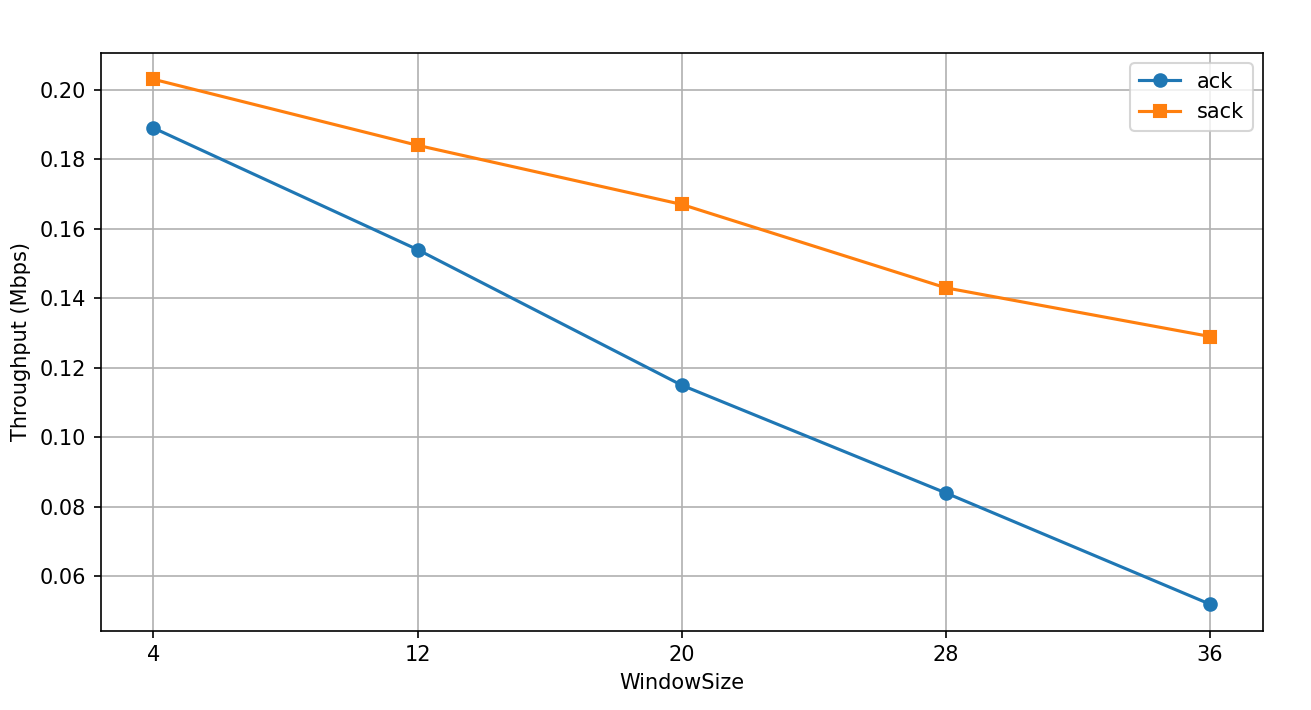
\includegraphics[width=0.8\textwidth]{img/p2.png}
    \caption{窗口大小对吞吐率的影响}
\end{figure}

可以看到,随着窗口大小增加,两种确认机制吞吐率都会往下跌。这也证实了并不是窗口越大,每次发送的数据越多,吞吐率就越高。事实上,理想状态下的窗口大小应该与延时带宽积差不多大小。同时随时窗口大小增加,累计确认的吞吐率严重下滑。这是因为一旦丢失了某个包后,需要重传整个窗口,造成带宽的大量浪费。而选择确认由于有失序缓存机制,相较来说影响会小一些。



\section{累计确认和选择确认的性能比较}
我们固定两者窗口大小仍为4,进行性能比较。依旧是固定变量,设置延时为0ms,改变丢包率得到图表:
\begin{table}[h!]
  \centering
  \begin{tabular}{|l|c|r|} % l=left, c=center, r=right
    \hline
    丢包率 & 累计确认    & 选择确认 \\ \hline
    2\% & 0.239Mbps & 0.226Mbps \\ \hline
    4\% & 0.161Mbps & 0.189Mbps \\ \hline
    6\% & 0.106Mbps & 0.167Mbps \\ \hline
    8\% & 0.083Mbps & 0.143Mbps \\ \hline
    10\% & 0.061Mbps & 0.129Mbps \\ \hline
  \end{tabular}
  \caption{累计确认和选择确认吞吐率对比}
  \label{tab:my_label}
\end{table}\par
\begin{figure}[H]
    \centering
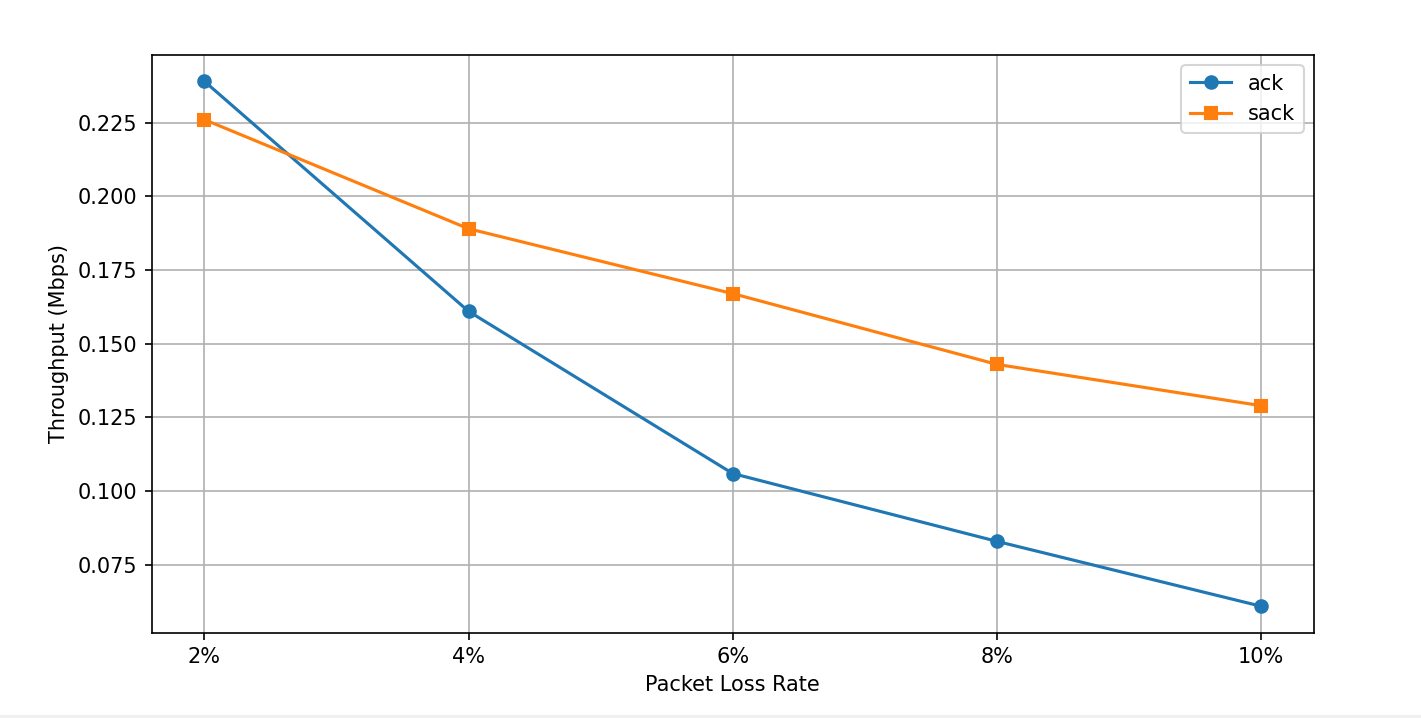
\includegraphics[width=0.8\textwidth]{img/p3-1.png}
    \caption{累计确认和选择确认吞吐率对比}
\end{figure}
再固定丢包率为0,改变延时,得到以下图表:
\begin{table}[h!]
  \centering
  \begin{tabular}{|l|c|r|} % l=left, c=center, r=right
    \hline
  延时    & 选择确认    & 累积确认      \\ \hline
  5ms	   & 0.438Mbps	& 0.451Mbps    \\ \hline
 10ms	& 0.402Mbps  & 0.405Mbps    \\ \hline
 20ms	& 0.335Mbps  & 0.327Mbps    \\ \hline  
 40ms	& 0.279Mbps	 & 0.287Mbps    \\ \hline
 60ms	& 0.242Mbps	 & 0.256Mbps    \\ \hline
 80ms	& 0.218Mbps  & 0.220Mbps    \\ \hline
100ms	 & 0.169Mbps  & 0.178Mbps    \\ \hline
  \end{tabular}
  \caption{累计确认和选择确认吞吐率对比}
  \label{tab:my_label}
\end{table}\par
\begin{figure}[H]
    \centering
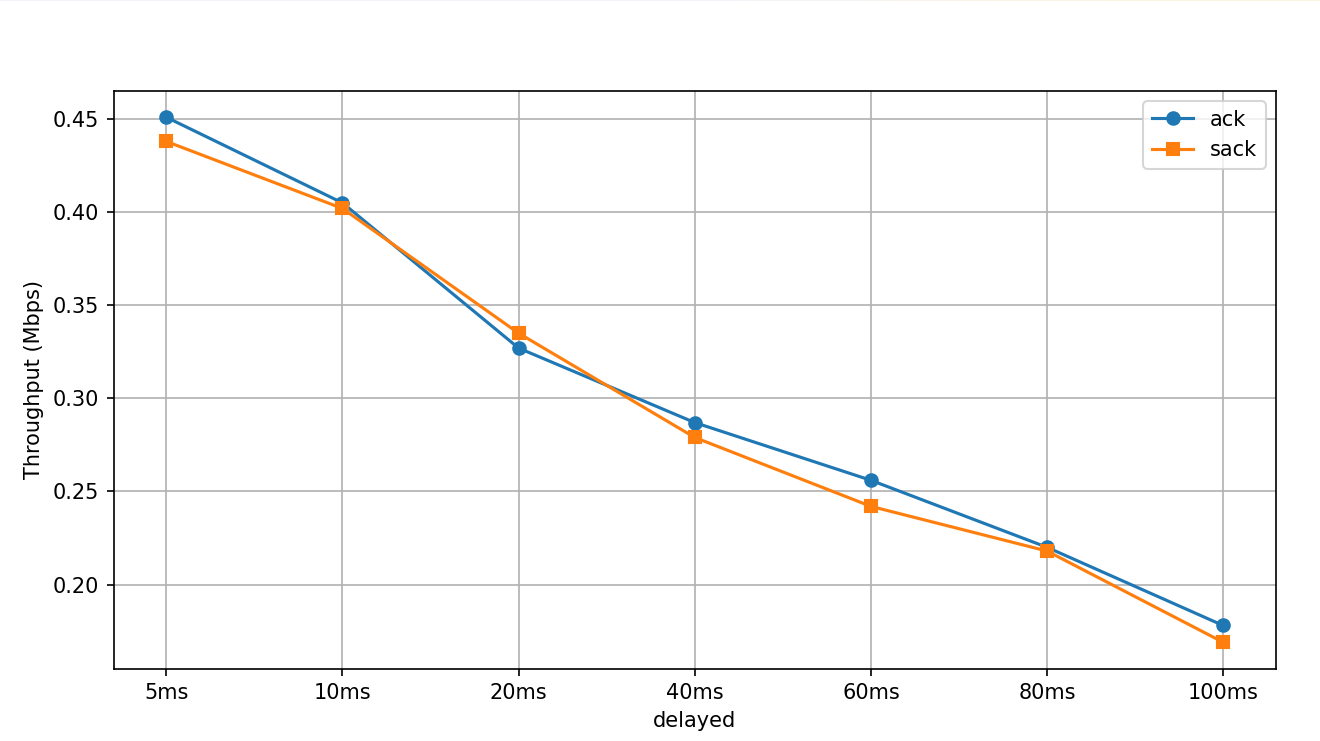
\includegraphics[width=0.8\textwidth]{img/p3-2.png}
    \caption{选择确认 vs 累计确认}
\end{figure}
从图中可以看到,当丢包率为2\%的时候,累计确认和选择确认的吞吐率相近,甚至累计确认还要再高一点(这一点可能是因为单次测量数据的误差引起的),但随着丢包率的增加,选择确认性能下降速度明显慢于累计确认,符合理论课所讲的知识。选择确认支持缓存失序数据包。单个包的丢失不会因为整个窗口的重传,而累积确认需要重传整个窗口。但延时对二者的影响几乎相同,二者吞吐率基本以相同的速率下降,这是因为选择确认针对的是缓存丢失的数据包。与之前的分析类似,延时增加 RTT 的值,在没有超过设定的超时时间的情况下,数据包基本不会丢失(除非底层UDP本身传丢了),故而选择确认的缓存机制也没有发挥作用。所以二者吞吐率基本相近。


\section{反思与总结}
通过本次实验,我才发现自己实现的滑动窗口还存在不足,尽管在代码逻辑上按照状态机和模型实现了相应的机制和功能,但并没有达到优化的效果,反倒是相较于停等协议性能会更差。这其实在工程学上也是一个很有意思的问题,如果在实现优化方案引入太多其他的开销(比如多线程、互斥锁等内容)或者实现方式不当,最后实际效果也许还不如最开始实现简单的方案。\par
同时我也发现,即使是同一台电脑上,同一丢包率和延时下传输同一文件,多次传输也会存在较大的性能差异。Socket 编程本质上还是调用操作系统实现的网络栈接口,这其中就涉及到线程调度、内存访问等多重因素影响,所以每次传输吞吐率存在差异。总之,通过本学期自己的实际编程体会,我发现网络传输具有较大的不确定性,与以往编写算法或者数据结构程序不同,每一次传输文件(执行程序)的时间可能都会有较大差异。在今后的学习中,争取能更深入地理解网络知识。

\end{document}
